\subsection{Overview}

ActivitySim is an agent-based modeling (ABM) platform for modeling travel demand. Like UrbanSim, the ActivitySim software is entirely open source, and hosted as a part of the Urban Data Science Toolkit at  https://github.com/UDST. ActivitySim grew in large part out of a need for municipal planning organizations (MPOs) to standardize the modeling tools and methods that were common between them in order to facilitate more effective collaboration and sharing of innovations. Today, ActivitySim is both used and maintained by an extremely active consortium of MPOs, transportation engineers, and other industry practitioners. Because of the cooperative approach taken by ActivitySim stakeholders towards its ownership, and because many of its "owners" are also its main users, the platform continues to mature in the direction that most benefits the practitioners themselves. ActivitySim development is still in Beta, with an official 1.0 release scheduled for 2018.

\subsection{Inputs}

ActivitySim requires two main sets of input data, one relating to geography and the other to the population of synthetic agents whose travel choices are being modeled. 
    
The geographic data is stored at the level of the traffic analysis zone (TAZ) and is comprised of three components: 1) land use characteristics; 2) a matrix of zone-to-zone travel impedances (travel times, distances, or costs) specific to the mode of travel and time of day; and 3) a table of user-defined measures of aggregate utility estimated for each zone. In transportation planning, the zone-level impedances and utility measures are commonly referred to as \textit{skims} and \textit{accessibilities}, respectively. 

Land use data consists of zone-level population and employment characteristics, along with measures of different land use and building types. We rely on UrbanSim ois read directly from UrbanSim outputs. It 

Travel skims are typically generated by a traffic assignment model, which ActivitySim is not. ActivitySim instead expects to load the skims from an OMX formatted data file [\textit{citation needed}]. The creation of these skims is described below in the section on traffic assignment.

Accessibilities can be generated directly from the skims or any other graph representation of the transportation network. They are computed by aggregating mode-specific measures of access to specific amenity-types across the network, most commonly employment centers, retail outlets, and transportation hubs. The measures of access can be as simple as counts of amenities accessible within a given shortest-path distance or travel time, or as complex as logsums generated by a discrete choice model. 

The second set of ActivitySim input data is the synthetic population. The synthetic population data consists of both individuals and their characteristics, as well as the households and household characteristics into which the individuals are organized. The synthetic population is shared between UrbanSim and ActivitySim, although UrbanSim does not make use of individual-level characteristics. 

The specifics (field names, file formats, etc.) of the ActivitySim data schema are well documented and available here [https://udst.github.io/activitysim/dataschema.html]

\subsection{How it works and what it does}

ActivitySim, like UrbanSim, relies heavily on discrete choice models and Random Utility Maximization theory \citep{mcfadden-1974}. Please refer to the relevant UrbanSim sections above for specific details about how discrete choice models work within an agent-based microsimulation framework.

An ActivitySim run consists of a series of model steps executed sequentially. The individual models can be grouped into the four clusters -- long term decisions, coordinated daily activity patterns, tour-level decisions, and trip-level decisions -- illustrated in Figure 7 and described below:
\begin{enumerate}[label=(\roman*)]
    \item \textit{Long Term Choice Models}: ActivitySim's three long-term choice models -- workplace location choice, school location choice, and auto-ownership -- model the choices that are not made every day in the real world but have an impact on those that are. These models will eventually be migrated to run directly from the UrbanSim environment so that the time horizons of the two simulation platforms are internally consistent.
    \item \textit{Coordinated Daily Activity Patterns}: The CDAP step models the group decision-making process for individual household members all seeking to maximize the utility of their daily activities together. CDAP takes into consideration mandatory and non-mandatory trips choosing activities to maximize each individual's utilties. The maximization process currently involves the estimation of all possible combinations of all individuals within a household, and is thus has the longest run-time of all ActivitySim models. 
    \item \textit{Tour-level Decisions}: Tours define chains of trips that are completed together without returning home in between. Mandatory tours include trips to and from work and school, while non-mandatory trips are entirely discretionary. Non-mandatory tour alternatives are specified in a user-defined configuration file, and thus these steps include a destination choice model as well. Mandatory tour alternatives have already been computed by the long term decision models. Each tour type has separate model steps for estimating mode choice, departure time, and frequency of the tour.
    \item \textit{Trip-level Decisions}: Mode choice must be selected at the level of the individual trip as well as the tour because a given tour may includes different modes for different trip legs. Trip departure and arrival times are estimated as well. The rest of the trip characteristics are inherited from the tours to which a trip belongs. 
\end{enumerate}

 
\begin{figure}[ht]
    \center
    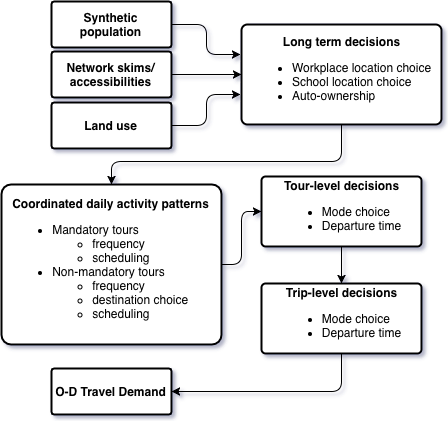
\includegraphics[width=\textwidth]{graphics/asim_flow.png}
    \caption{ActivitySim model flow adapted from http://analytics.mtc.ca.gov/foswiki/bin/view/Main/ModelSchematic}
    \label{fig:asim-models}
\end{figure}

\subsection{Outputs}

The output of an ActivitySim run consists of a single HDF5 data file with a single table of results corresponding to each model step, along with the versions of the input files in their final, updated states. For the purpose of generating travel demand for traffic assignment, however, we are only concerned with the output of the trip generation step. This single file contains the origin and destination zones, start and end times, and mode choice for every trip taken by every agent over the course of a day. We then take the subset of these trips that are completed by automobile and aggregate the counts by origin-destination pair and hour of departure. These hourly, zone-level demand files are finally handed off for use in traffic assignment.

\subsection{Calibration and validation}

